\documentclass[../AnalysisNoteJBuxton.tex]{subfiles}
\begin{document}

\subsection{Pair Selection}
\label{PairSelection}

Some general remarks on forming pairs

It is important to obtain true particle pairs in the analysis.  In particular, contamination from pairs constructed with split or merged tracks can introduce an artificial signal into the correlation function, obscuring the actual physics.

\begin{figure}[h]
  \centering
  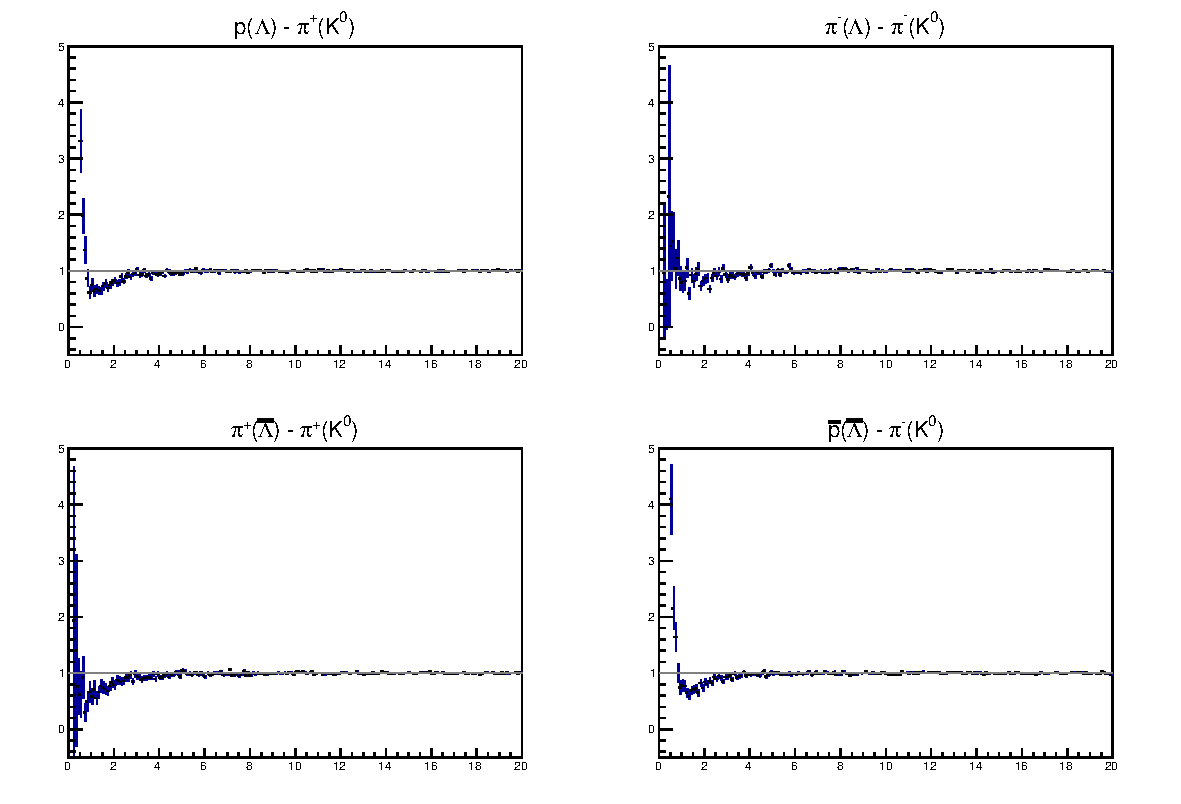
\includegraphics[width=0.8\textwidth]{3_DataSelection/Figures/AvgSepCFs_LamK0.pdf}
  \caption[Avgerage Separation of $\Lambda$($\bar{\Lambda}$) and K$^{0}_{S}$ Daughters]{Avgerage Separation of $\Lambda$($\bar{\Lambda}$) and K$^{0}_{S}$ Daughters.  Only like-sign daughter pairs are shown (the distributions for unlike-signs were found to be flat).  The title of each subfigure shows the daughter pair, as well as the mother of each daughter (in ``()"),  ex. top left is p from $\Lambda$ with $\pi^{+}$ from K$^{0}_{S}$.}
  \label{fig:AvgSepLamK0}
\end{figure}

\begin{figure}[h]
  \centering
  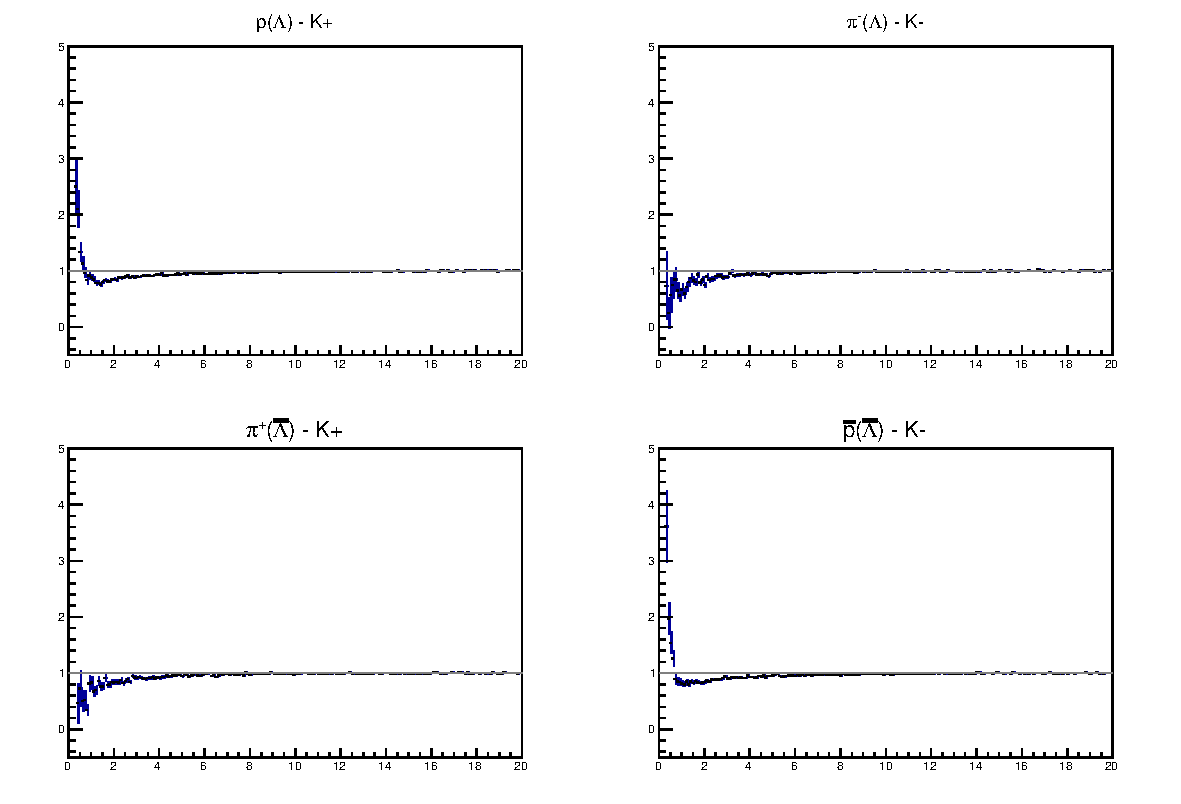
\includegraphics[width=0.8\textwidth]{3_DataSelection/Figures/AvgSepCFs_LamKch.pdf}
  \caption[Avgerage Separation of $\Lambda$($\bar{\Lambda}$) Daughter and K$^{\pm}$]{Avgerage Separation of $\Lambda$($\bar{\Lambda}$) Daughter and K$^{\pm}$.  Only like-sign pairs are shown (unlike-signs were flat).  In the subfigure titles, the particles in ``()" represent the mothers, ex. top left is p from $\Lambda$ with K$^{+}$.}
  \label{fig:AvgSepLamKch}
\end{figure}

\end{document}